\section{Thursday, May  8: Clustering Day 2: Spectral Clustering and the problem of Validation}

\subsection{What is Spectral Clustering, and why might we use it?}

Figure~\ref{compact_connect} shows a classic picture that motivates spectral clustering. It is just a toy example: in real life, our data has more than 2 dimensions and it probably does not look like donuts! But it is still a helpful motivator. 

The idea is that K-means and other clustering algorithms that use Euclidean distance as a similarity metric will do really poorly on the donut-shaped data. The donut-shaped data shows that we don't always want to prioritize compactness in defining clusters; sometimes we want to prioritize connectivity. This is where graph-based clustering methods can be really useful. Spectral clustering is an example of a graph-based clustering method. 

The biggest and most important ideas behind spectral clustering are things that you could have come up with earlier in the semester. One big idea is that we can use distance-metrics besides Euclidean distance! Another big idea is that we can take data that doesn't initially look ``nice," and make it look nice by expressing it in new coordinates (we did this with transformations, SVM kernels, etc.) A final big idea (that was maybe under-emphasized early in the semester) is that linear algebra is really cool and magical. 

For spectral clustering, we can make a similarity matrix for our data points that calls two points similar if they are in each-other's K nearest neighbors. This might have Euclidean distance hiding underneath (if we use Euclidean distance to define our K nearest neighbors), but you can tell from looking at the right panel of Figure~\ref{compact_connect} that this similarity metric will do quite well on the donut-shaped data-- it will know that all of the red points are ``neighbors by transitive property," but none of the blue points are ``connected" to any red points. This similarity matrix is $n * n$ and symmetric: element $i,j$ stores the similarity between object $i$ and object $j$. It should be non-negative. We put $0$s on the diagonal (element $i$ is not marked as being similar to itself). This similarity matrix is $S$. There are all sorts of ways to define it: we don't need to use KNN. We could use KNN weighted by Euclidean distance, just Euclidean distance, etc. 

Another cool thing is that we don't need to start with numerical data; we can start with something like text data! We can make a similarity matrix between words in our ``dictionary" by counting the number of times that the words co-occur in a sentence or document. We can then apply spectral clustering to this similarity matrix: this is really widely used in practice!

This similarity matrix can be seen as the adjacency matrix of a graph representation of our dataset. Our new notion of clusters is cliques in this graph: either perfectly connected components, or else groups of nodes with a lot of edges (or a lot of highly weighted edges) between them that are connected to OTHER groups of nodes by very few edges. 

Once we have our similarity matrix $S$, we make our degree matrix $D$, which just stores the row sums of $S$ on its diagonal. It expresses overall connectedness of a point $i$ with element $i,i$. Finally, we let $L = D-S$. This is the Laplacian matrix of our graph representation of our data.

Finally, we take an eigen-decomposition of $L$. We know that we have one eigenvector of $0$, because the rows of $L$ must sum to $0$ by construction, and so the matrix does not have full rank (the vector of all $1$s is in the null space). The multiplicity of $0$ as an eigenvector is the number of perfectly connected components of the graph. The idea is that, to find clusters that are not perfectly connected components, we can run k-means on a few of eigenvectors of $L$ corresponding to the small (but non-zero) eigenvalues. 

Why did we do all of this work if we were just going to be applying K-means? Because we are now applying K-means to a transformed version of our data. This is like the kernel trick for SVMs! We took data that looked like donuts, and in these new coordinates (it's just a transformation!), it will look like something that K-means can cluster. This is so cool!

All we did was transform our data, but it turns out that small eigenvectors of the $L$ matrix give an optimal transformation if our goal is to represent connected components as compact components! Linear algebra is so cool! Feel free to play around with the R demo on GLOW!

You might notice that there are still a LOT of choices involved in running spectral clustering. The final choice of $K$ for $K$-means. The dimension of the spectral embedding (how many eigenvectors to use in the transformed version of the data). The distance metric for the initial similarity matrix. Etc. Since we have no ground truth, it is really hard to know how to pick these things!

So, despite having seen a few different types of clustering at this point, we are still left with one basic question: how do we know which clustering is best among a set of candidate options?

We need to be able to do model selection and model validation for clustering!!!


\begin{figure}
\centering
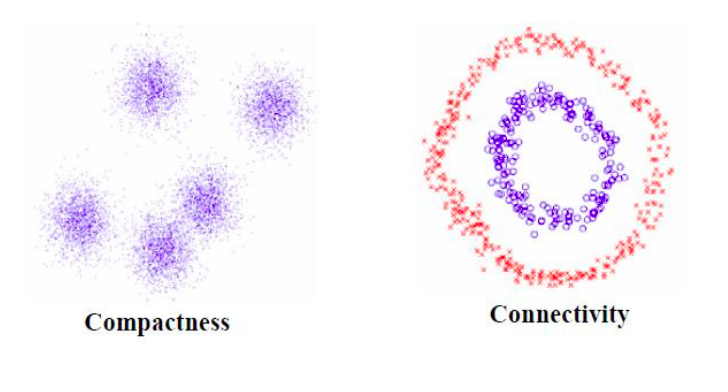
\includegraphics[width=0.7\textwidth]{442_lecs/compactconnect.png}	
\caption{This figure shows two different notions of ``good clusters" or ``similarity" in two dimensions. On the left, we see 5 clusters that are ``good" according to a classic notion of compactness: k-means will be great for identifying these five clusters. Euclidean distance in untransformed space captures the structure in the data! On the right, we see concentric circles. K-means will be terrible at identifying these two clusters, but a graph-based approach (like spectral clustering) with the right similarity metric will do great!}
\label{compact_connect}
\end{figure}


\subsection{How can we do model validation for clustering?}

Unfortunately, this is really hard. See the slides that I posted on GLOW.

Big picture, we could try to evaluate a clustering using something like within-cluster mean-squared error. This choice of loss function makes a lot more sense in the K-means world, where we are prioritizing compactness. 

It should not surprise you all to know that within-cluster MSE will always decrease (on a training set) when we increase $k$, the number of clusters. This is because of overfitting: a model with $10$ clusters can ``fit" the data better than a model with $5$ clusters; however, it might just be fitting noise, not signal.

In the supervised setting, we avoid issues of overfitting by splitting our data into training and test sets. Unfortunately, this does not work well for clustering! The problem is that, if we cluster a training set, we have nothing to evaluate on the test set! Clustering a training set does not yield an equation that can be easily applied to a test set to obtain cluster labels for a test set, and it does not provide cluster labels for the test set. This is the fundamental difficulty! 

Because of this difficulty, in unsupervised learning people often do not strive for nice, U-shaped loss functions that are minimized at the best value of $k$. Instead, they look for elbow-shaped loss functions, where a visible ``elbow" in the loss function curve at $k$ clusters tells us that, past $k$, we are likely fitting noise and not signal. 

This ``elbow method" is widely used, but leaves much to be desired! An active area of work over the past 20 years has been trying to formalize the elbow method or else come up with alternate ways to do cross validation that work for unsupervised learning. 


\section{Monday, May 12: Dimension reduction and recommender systems}

We have used principle components or the SVD a few times this semester, but I haven't really told you very many details about them! Today, we will study the singular value decomposition of a matrix in a little more detail. We will then touch on some really cool applications of the SVD and other matrix decompositions. 

The theme for today: unsupervised learning is more than just clustering! There are other task that involve finding structure in unlabeled data!

\subsection{What is the SVD?}

We can decompose any $X \in \mathbb{R}^{n \times p}$ into
$$
X = U D V^T.
$$
Without loss of generality, assume that $n \times p$. Then $U$ is an $n \times p$ matrix where the columns are orthogonal unit vectors; $D$ is a diagonal $p \times p$ matrix; $V$ is a $p \times p$ orthonormal matrix. The diagonal elements of $D$ are nonnegative, and $D_{11} \geq D_{22} \geq D_{33} \ldots$. These values in $D$ are called the singular values of $X$. 

Because of the properties above, $U^T U = I_p$, $V^T V = I_p$, $VV^T = I_p$, but  $UU^T \neq I_n$. 

\subsection{What are the uses of the SVD?}

For the purposes of today, here is the cool thing about the SVD. If you want to approximate $X$ with a rank-$k$ alternative, where $k << p$, then the best possible approximation (in terms of SSE) is:
$
U_k D_{k} V_{k}^T
$, where $U_k$ represents the first $k$ columns of $U$, $D_k$ represents the top $k \times k$ block of $d$, and $V_k$ is the first $k$ columns of $V$. 

We interpret the columns of $V$ as our new axes in a new, transformed space where we need less information to express $X$. The coordinates of the data points along these new axes are given in $U D$; they represent the projection of $X$ into the axes defined by $V$. It turns out that this is an optimal projection/transformation: $U_k D_{k} V_{k}^T$ is as close as we can get to representing $X$ if we only want to store $k$ components instead of $p$. 

This tells us that, if we want to do dimension-reduction and we care about how close our reduced-dimension version of our data is to $X$, we should do the SVD! 

Why would we want to do dimension-reduction?

\begin{itemize}
\item As preprocessing for supervised learning (on the predictors), to avoid the curse of dimensionality or redundant predictors. 
\item As preprocessing for clustering, to avoid the curse of dimensionality or redundant predictors. 
\item To de-noise our data, or store a cheaper version of our data (i.e. image compression). This is a truly unsupervised task. 
\item To uncover latent factors in our data. We can interpret the columns of $V$ as defining new variables: these might be interpretable for us! This is a true unsupervised / ``finding structure" task. 
\end{itemize}

For any of these applications: deciding $k$, the latent dimension, is JUST as hard as picking the number of clusters. We have no good cross-validation-ish solution! Because it is unsupervised! We can make things like elbow plots. You did this on your HW! 

These are applications that I think you have encountered before. Today, we will at least partially cover matrix completion and missing data, which is an extension that I don't think you have seen before!

\subsection{How does this relate to principal components and eigenvalues?}

If you take your data matrix $X$ and you center and scale it so that each column has mean $0$ and standard deviation $1$, then the SVD gives exactly PCA. The columns of $V$ are the loading vectors, and the columns of $UD$ are the score vectors. 

If $X = UD V^T$, then $X^T X = V D^2 V^T$. $X^T X$ is a symmetric, square matrix. It turns out that $V D^2 V^T$ is exactly the spectral decomposition of the matrix $X^T X$: The diagonal elements of $D^2$ are the eigenvalues of $X^T X$ and the columns of $V$ are the eigenvectors of $X^T X$.

This perhaps helps you relate the SVD to previous things that you learned about PCA. If $X$ is centered and scaled, then $X^T X$ is the correlation matrix of $X$. The leading eigenvectors of the correlation matrix tell you the directions of maximum variation in $X$; these are the top principal components. Today, you saw that you can obtain these same directions using the SVD. 

I think it's generally good to know that eigenvectors are directions of maximum or minimum variance (depending on if they go with the smallest or the largest eigenvalues), and that singular vectors are the best ways to reconstruct a dataset faithfully in fewer dimensions. I did not retain this after Math 250 at Williams, but I learned it eventually!

\subsection{Recommender Systems}

This is the application that I want to focus on today, because I think it is unlikely that you have seen it in a previous course, and I think that it is a beautiful application of linear algebra to an important problem.

Suppose that I work for Netflix, and you are a customer of Netflix. You have a viewing/rating history on Netflix, and I also have viewing/rating histories for tons of other users. I want to predict if you will enjoy movie $j$.

This sounds like a supervised task. I want to make a prediction! But there is a problem with the availability of data.

Suppose that I would like to use the predictions from past customers who rated movie $j$ to predict your rating for movie $j$. Well, I can only include customers who actually watched/rated this particular movie. I also need to know which of these customers is ``similar" to you, so I need you to have watched and rated similar previous movies to these customers. If I try to approach this in a totally supervised manner, I am going to need to really cut down on my dataset size. And ... I will need to do this for every movie and every user separately? This sounds terrible!

While this task sounds fundamentally supervised (predict a movie rating), it turns out to have a really nice solution via unsupervised learning. 

Let $X$ be a matrix with $n$ rows for $n$ total Netflix customers and $p$ columns for $p$ total movies on Netflix. Let $X_{ij} = r_{ij}$, a rating, if customer $i$ rated movie $j$. Otherwise, let the value $X_{ij}$ be missing.

Our goal is to fill in the missing entries in the matrix with our best guesses that respect the structure of the data. We can then use the imputed value for $i,j$ to be the predicted rating for user $i$ and movie $j$: and use this to decide if we should recommend movie $j$ or not. This is known as matrix completion! 

We do this under the assumption that $X$ (if it had no missing values) would be well-approximated with a \emph{low rank} structure, where $X \approx U_kD_k V_k^T$. The latent axes ($V$) are latent genres of movies (the column space of $X$) and the coordinates in $U$ define latent cliques of users (the row space of $X$). 

If $X$ had no missing values, we would directly apply the $SVD$ to find our latent genres and cliques. Which could be a cool exercise in ``understanding the structure in our data," latent variable modeling, etc. So this is a general way in which the SVD could be interesting! But ... here we are in a very different situation, because probably 99\% of the matrix $X$ is missing values (in the case of the Netflix data). Standard computational techniques for computing the SVD cannot be applied!!

The general idea is that we want to solve the optimization problem:
$$
\mathrm{minimize}_Z \sum_{i,j \mathrm{observed}} (X_{ij} - Z_{ij})^2 \ \ \ \ \ \text{subject to: } rank(Z)=k. 
$$
If you could come up with this matrix $Z$, you would then have the SVD that you need to impute the missing entries! Unfortunately, this is really computationally hard to solve! But people have come up with nice approximations, algorithms, etc. 

ISL, Algorithm 12.1, covers ``Hard Impute", which I think is clever and makes sense and is an awesome demonstration of how learning fundamentals like the SVD and seemingly ``dumb" solutions (try something over and over with slightly improved guesses) can really get you a long way. However, in practice, more complicated algorithms certainly exist too. 

The idea of Hard Impute is to start by guessing that every missing value in $X$ is equal to its column mean. So, if a user has not rated a movie, assume that they would rate it as the average of all other users. Call this guessed-matrix $\tilde{X}$, and compute the SVD of $\tilde{X}$. Then, replace every MISSING element in $X$ with its low-rank approximation (you need to have already picked the rank) suggested by the SVD of $\tilde{X}$. Repeat this process over and over until your reconstruction error on your OBSERVED entries stops decreasing. 

You might enjoy reading about the Netflix Prize \\ (\url{https://www.thrillist.com/entertainment/nation/the-netflix-prize})
 of the early 2010s, which is when this problem and this field really took off! Also, the paper that discusses Hard Impute (\url{https://www.jmlr.org/papers/volume11/mazumder10a/mazumder10a.pdf}) also discussed L1 regularized versions that might be preferable. 
 
\section{Thursday, May 15: Final presentations}

The end! No more lecture notes! Hopefully these lecture notes will improve a lot between now and the next time I teach this class (summer project!). 



